\documentclass[11pt,fleqn]{exam}
\usepackage[utf8]{inputenc}
\usepackage[T1]{fontenc}
\usepackage{fancyvrb}
\usepackage{amsmath}
\usepackage{amssymb}
\usepackage{amsthm}
\usepackage{hyperref}
\usepackage{algpseudocode}
\usepackage{comment}
\usepackage{enumitem}
\usepackage[margin=0.75in]{geometry}
\usepackage{tikz}
\usetikzlibrary{arrows,arrows.meta,positioning,intersections,shapes.gates.logic.US,calc}
\algnewcommand\algorithmicforeach{\textbf{for each}}
\algdef{S}[FOR]{ForEach}[1]{\algorithmicforeach\ #1\ \algorithmicdo}
\newcommand{\fillinMCmath}[1]{
\begin{tikzpicture}\draw circle [radius=0.5em];\end{tikzpicture}\ #1}
\newcommand{\fillinMCmathsoln}[1]{
\begin{tikzpicture}\draw[black, fill=blue] circle [radius=0.5em];\end{tikzpicture}\ #1}
\newcommand{\ptsamt}[1]{[#1~points]}
\newcommand{\ptamt}[1]{[#1~point]}

%%% Adding Colour to Questions and Answers
\usepackage{color}

\definecolor{solnblue}{rgb}{0,0,1}
\newenvironment{soln}{\color{solnblue}}{}

%Questions

% Answers
\definecolor{blu}{rgb}{0,0,0.5}
\def\blu#1{{\color{blu}#1}}
\definecolor{gre}{rgb}{0,.3,0}
\def\gre#1{{\color{gre}#1}}
\definecolor{red}{rgb}{0.5,0.0,0}
\def\red#1{{\color{red}#1}}
\def\norm#1{\|#1\|}
%%% End for Colours

%fancyvrb commands
\def\lar{$\leftarrow$}
\def\lesseq{$\leq$}


% \newif\ifsolutions\solutionstrue
\newif\ifsolutions\solutionsfalse

\makeatletter

\ifsolutions
\title{COSC 320: Assignment 2 Solutions}
\else
\title{COSC 320: Assignment 2}
\fi
\author{}
\date{}
\hypersetup{
  pdfkeywords={},
  pdfsubject={},
  pdfcreator={Emacs Org-mode version 7.9.3f}}

\begin{document}

\maketitle
\vspace{-0.5in}

\ifsolutions
\setcounter{section}{1}
\else
This assignment is due \textbf{Friday, February 7 at 7 PM}. Late submissions will not be accepted. All the submission and formatting rules for Assignment~1 apply to this assignment as well.  
%------------------------------------------------------------------------------------
\begin{enumerate}
   \item Rin Meng, 51940633
   \item Mika Panagsagan 29679552
	\item Kevin Zhang 10811057
\end{enumerate}
\section{List of names of group members (as listed on Canvas)}

Provide the list here. This is worth 1 mark. Include student numbers
as a secondary failsafe if you wish.

\section{Statement on collaboration and use of resources}
To develop good practices in doing homeworks,
citing resources and acknowledging input from others, please complete the following.
This question is worth 2 marks.

\begin{enumerate}
\item All group members have read and followed the guidelines for groupwork
on assignments given in the Syllabus).

\fillinMCmathsoln{Yes} \hspace{.5in} \fillinMCmath{No}

\item We used the following resources (list books, online sources, etc. that you consulted):
\begin{enumerate}
   \item DeepSeek R1, ChatGPT to generate ideas, explain concepts, and check if we are going in the right direction.
   \item Google Search, Google's AI Overview
   \item COSC 320 Lecture Slides
\end{enumerate}
\item One or more of us consulted with course staff during office hours.

\fillinMCmath{Yes} \hspace{.5in} \fillinMCmathsoln{No}

\item One or more of us collaborated with other CPSC 320 students; none of us took
      written notes during our consultations and we took at least a half-hour break afterwards.

\fillinMCmath{Yes} \hspace{.5in} \fillinMCmathsoln{No}

      If yes, please list their name(s) here:

\item One or more of us collaborated with or consulted others outside of COSC 320; none of us took written notes during our consultations and we took at least a half-hour break afterwards.

\fillinMCmath{Yes} \hspace{.5in} \fillinMCmathsoln{No}

      If yes, please list their name(s) here:

\end{enumerate}
\newpage
\fi

%==========================================

\section{Logarithmic functions grow more slowly than "polynomial" functions}

The textbook (2.8, page 41) provides the following useful fact, stating roughly that logarithmic functions are big-$O$-upper-bounded by
simple "polynomial" functions, specifically functions that are $n$ to some constant power:

\begin{quote}
{\bf Fact:} \emph{For every $b > 1$ and every $x > 0$, we have $\log_b n = O(n^x)$.}
\end{quote}

\begin{questions}
\question[4]
Use the fact above to prove the stronger assertion that logarithmic functions of $n$ grow strictly more slowly, in the little-$o$ sense, than
functions that are $n$ to some constant power:
\begin{quote}
\emph{For every $b > 1$ and every $x > 0$, we have $\log_b n = o(n^x)$.}
\end{quote}

  \ifsolutions
    \input{q2a-sol.tex}
\else
If you want, you can start your proof as follows:

\begin{soln}

\begin{proof}
   Now we want to show that:
   \[ \lim_{n \rightarrow \infty} \frac{\log_b n}{n^x} = 0 \]
   Fix $b>0$ and $x>0$. Using the fact, and since $x/2>0$, it must be the case that $\log_b n = O(n^{x/2})$.
   This means that there exists a constant $c>0$ such that for all $n$ sufficiently large, we have $\log_b n \leq c n^{x/2}$.
   Now we can write:
   \[ \frac{\log_b n}{n^x} \leq \frac{cn^{x/2}}{n^x} = \frac{c}{n^{x/2}} \]
   Now we can see that:
   \[ \lim_{n \rightarrow \infty} \frac{c}{n^{x/2}} = 0 \]
   Therefore, by the limit comparison test, we have that:
   \[ \lim_{n \rightarrow \infty} \frac{\log_b n}{n^x} \leq \frac{c}{n^{x/2}} = 0 \]
   $therefore$, we have shown that $\log_b n = o(n^x)$.
   
\end{proof}


\end{soln}
\fi

\question[4]
Now use the fact of part 1 to show that $\sqrt{n} = o(n/\log^3 n)$. Here the log is to the base 10, and $\log^3 n = (\log n)^3$.

\begin{soln}
   \begin{proof}
      We wish to show that 
      \[
      \sqrt{n} = o\left(\frac{n}{\log^3 n}\right),
      \]
      which, by definition, means that
      \[
      \lim_{n \to \infty} \frac{\sqrt{n}}{n/\log^3 n} = 0.
      \]
      Notice that
      \[
      \frac{\sqrt{n}}{n/\log^3 n} = \frac{\sqrt{n}\,\log^3 n}{n} = \frac{\log^3 n}{\sqrt{n}}.
      \]
      By the fact from part 1, for every base \(b > 1\) and every exponent \(x > 0\), we have 
      \[
      \log_b n = o\left(n^x\right).
      \]
      In particular, for \(b = 10\) and \(x = \frac{1}{3}\) we obtain
      \[
      \log^3_{10} n = o\left(n^{1/3 \times 3/2}\right) = o\left(n^{1/2}\right).
      \]
      If 
      \[
         \frac{log^3_{n}}{\sqrt{n}} = \frac{o(n^{1/2})}{o^{1/2}} = o(1)
      \]
      Based on the limit,
      \[
      \lim_{n \rightarrow \infty} \frac{\log^3 n}{\sqrt{n}} = 0,
      \]
      $\therefore$ We have shown that $\sqrt{n} = o(n/\log^3 n)$.
   \end{proof}
\end{soln}



\ifsolutions
  \input{q2b-sol.tex}
\fi
\end{questions}

%==========================================
\clearpage

%===============================================================
\section{Counting Shortest Paths}

Let $G=(V,E)$ be an undirected, unweighted, connected graph with node set $\{1,2,\ldots,n\}$, where $n\ge 1$. For any node $v$, let $c(1,v)$ be the total number of shortest paths (i.e., paths with the minimum number of edges) from $1$ to $v$.

\vspace{.1in}

\noindent {\bf Example:} The following graph has one shortest path from 1 to 6. Also there are three shortest paths from 1 to 8. Two of these,
namely path 1,2,3,8, and path 1,6,3,8, go through node 3, while one, namely path 1,6,5,8 goes through node 5.

\vspace{.1in}

% \hspace{.5in} \includegraphics[width=0.3\textwidth]{a2-graph1.pdf}

\vspace{.1in}

\begin{questions}
\question[2]
Draw a breadth first search tree rooted at 1 for the graph above. Include all dashed edges as well as tree edges. (A scanned hand-drawn figure is fine as long as it is clear.)

\begin{soln}
   % \hspace{.5in} \includegraphics[width=0.25\textwidth]{q4soln.png}
   \begin{tikzpicture}
      % Define nodes
      \node[circle, draw, ] (1) at (2,2) {1};
      \node[circle, draw,] (2) at (0,0) {2};
      \node[circle, draw,] (3) at (0,-2) {3};

      \node[circle, draw,] (6) at (4,0) {6};
      \node[circle, draw,] (4) at (4,-2) {4};
      \node[circle, draw,] (7) at (4,-4) {7};
      \node[circle, draw,] (5) at (6,-2) {5};
      \node[circle, draw,] (8) at (6,-4) {8};
    
      % Draw edges
      \draw[-] (1) -- (2) node[midway, above] {};
      \draw[-] (1) -- (6) node[midway, above] {};
      \draw[-] (2) -- (3) node[midway, above] {};
      \draw[-] (6) -- (4) node[midway, above] {};
      \draw[-] (6) -- (5) node[midway, above] {};
      \draw[-] (5) -- (8) node[midway, above] {};
      \draw[-] (4) -- (7) node[midway, above] {};
      \draw[dashed] (3) to[out=-100, in=220] (8);
      \draw[dashed] (3) to[out=-50, in=200] (7);
      \draw[dashed] (3) -- (6) node[midway, above] {};
      \draw[dashed] (4) -- (5) node[midway, above] {};
    \end{tikzpicture}
\end{soln}


\ifsolutions
\begin{soln}
% \hspace{.5in} \includegraphics[width=0.25\textwidth]{Counting-SPs-bfs.pdf}
\end{soln}
\else
\fi

\question[2]
How many shortest paths are there from node 1 to node 7? That is, what is the value of $c(1,7)$? Give a list of the paths.
\vspace{.1in}

\begin{soln}
   \[ 
   c(1,7) = 3 \text{ with paths } \{1,2,3,7\}, \{1,6,3,7\}, \{1,6,4,7\}
   \]
\end{soln}

\ifsolutions
\begin{soln}
$c(1,7) = 3$, and the three paths are 12,3,7; 1,6,3,7; and 1,6,4,7.
\end{soln}
\else
\fi

\ifsolutions
\clearpage
\fi

\question[4]
\label{counting-alg}
Here is an inductive definition for $c(1,v)$: The base case is when $v=1$, in which case we define $c(1,1)$ to be 1, since there is exactly one shortest path from $1$ to itself (with no edges). When $v > 1$, let $d[v]$ be the depth of any node $v$ in the bfs tree of $G$ rooted at 1. Then
\[
c(1,v) = \sum_{\begin{array}{l}u \;|\; (u,v) \in E, \mbox{ and} \\ d[u] = d[v] - 1\end{array}} c(1,u).
\]
Intuitively, on the right hand side we are summing up the number of shortest paths from node 1 to all nodes $u$ at level $d[v]-1$, such that there is an edge of $G$ (either a tree edge or a dashed edge) from $u$ to $v$. In our example above, $c(1,8) = c(1,3) + c(1,5)$.

Provide code in the spaces indicated below, that leverages this inductive definition to obtain an algorithm that computes $c(1,v)$ for all nodes $v$. This code first initializes $c(1,v)$ for all $v$, and then calls a modified version of breadth first search that you will flesh out.

\vspace{,1in}

\ifsolutions
\input{q3a-sol}
\else
\begin{algorithmic}
 \Procedure{Count-Shortest-Paths}{$G$.1}
    \State $\triangleright$ $G$ is an undirected, connected graph with nodes $\{1,2,\ldots,n\}$, where $n \ge 1$
    \State $\triangleright$ compute $c(1,v)$, the number of shortest paths, from 1 to $v$, for all nodes $v$
     \State $\triangleright$ {\bf add code here to initialize $c(1,v)$ for all $v \in V$}:
      \begin{soln}
         \For{each node \(v \in V\)}
         \State \(c(1,v) \gets 0\)
      \EndFor
      \State \(c(1,1) \gets 1\)  \Comment{There is exactly one shortest path from 1 to itself.}
      \end{soln}
      \State call \textsc{Modified-BFS}($G$)
\EndProcedure
\end{algorithmic}

\vspace{.1in}

 \begin{algorithmic}
\Procedure{Modified-BFS}{$G$}
\State $\triangleright$ Assume that this procedure can access and update the variables $c(1,v)$
\State add node $1$ as the root of the bfs tree
\State $d[1] \gets 0$ \Comment node 1 is at level 0
\For{all nodes $v > 1$}
   \State $d[v] \gets \infty$ \Comment $v$ is not yet in the tree
\EndFor
\State $d \gets 1$
\While{not all nodes are added to the tree}
   \For{each node $u$ in the tree with $d[u] = d-1$}
      \For{each $v$ adjacent to $u$}
        \If{$d[v] == \infty$} \Comment $v$ has not yet been added to the tree
           \State $d[v] \gets d$  \Comment put node $v$ at level $d$ of the tree (as a child of $u$)
        \EndIf
            \State $\triangleright$ {\bf add your code here to update $c(1,v)$}:
            \begin{soln}
               \If{\(d[v] == d\)} \Comment update the count if \(v\) is at the current level \(d\)
                  \State \(c(1,v) \gets c(1,v) + c(1,u)\)
               \EndIf
            \end{soln}
\EndFor
   \EndFor
   \State $d \gets d+1$        
\EndWhile
\EndProcedure
  \end{algorithmic}
   \fi   
 \end{questions}

\clearpage

%===============================================================

\section{Provision planning}
You run a business to provide provisions to individuals with plans
for long-distance hikes. An individual requesting your help tells you:
\begin{itemize}
\item
$d$: The distance (in km) that the individual can hike per day, where $d$ is a positive integer;
\item
$p$: How many days of provisions (food, water, etc.) they can carry, where $p$ is a positive integer.
\end{itemize}
In addition you have access to:
\begin{itemize}
\item
$R[1..k]$: inter-town distances along the planned route, with $k \ge 1$. That is,
there are $k+1$ towns along the route with town 0 being the start and
town $k$ being the destination; and $R[i]$ is the distance (in km)
from town $i-1$ to town $i$ for $1\le i \le k$.
\end{itemize}
You need to store provisions in towns along the way,
that the hiker will pick up en route.  For this problem, you
need only concern yourself with instances $(d,p,R[1..k])$ that have
valid solutions. A
{\em valid solution} is a list of towns where provisions can
be placed, so as to ensure that the hiker will not run out of
provisions. In a valid solution, the distance traveled between the starting town
and the first town in the solution, or between a consecutive pair of
towns in the solution, or between the last town in the solution and
the destination, is $\le dp$ (where $d$ and $p$ are defined above).
You never need to provide provisions at town 0 or town $k$ (the hiker
has their own provisions at the start of the trip and does not need
them once the destination is reached).  You want to find an {\em
  optimal solution}, that is, a valid solution of minimum length.

\vspace{.1in}
\noindent
{\bf Example}: A hiker plans to
hike for at most 7km per day, and can carry provisions that
last for two days, so $d=7$ and $p=2$.
Also, $k=5$ and $R[1..5] = [8,2,2,10,5]$, so distances between towns are:

\begin{center}
% \includegraphics[width=0.6\textwidth]{greedy-example1.png}
\end{center}
One valid solution is the list of towns 1, 3, 4:
\begin{center}
% \includegraphics[width=0.6\textwidth]{greedy-example1b.png}
\end{center}

\begin{questions}
\question[3]
In the example above, the solution is not optimal. Give {\em three
different optimal solutions}, which have only two towns in each.

\begin{soln}
    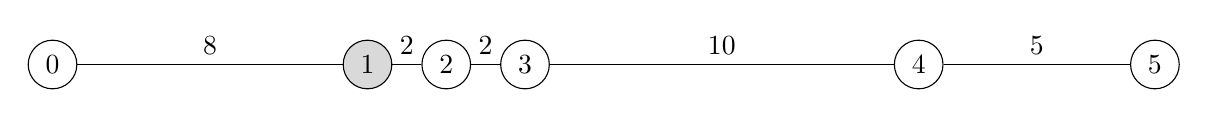
\begin{tikzpicture}
      % Define nodes
      \node[circle, draw, ] (0) at (0,0) {0};
      \node[circle, draw, fill=gray!30] (1) at (4,0) {1};
      \node[circle, draw,] (2) at (5,0) {2};
      \node[circle, draw,] (3) at (6,0) {3};
      \node[circle, draw,] (4) at (11,0) {4};
      \node[circle, draw,] (5) at (14,0) {5};
    
      % Draw edges
      \draw[-] (0) -- (1) node[midway, above] {8};
      \draw[-] (1) -- (2) node[midway, above] {2};
      \draw[-] (2) -- (3) node[midway, above] {2};
      \draw[-] (3) -- (4) node[midway, above] {10};
      \draw[-] (4) -- (5) node[midway, above] {5};
    \end{tikzpicture}

      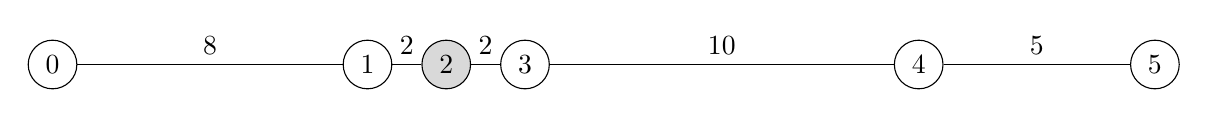
\begin{tikzpicture}
         % Define nodes
         \node[circle, draw, ] (0) at (0,0) {0};
         \node[circle, draw,] (1) at (4,0) {1};
         \node[circle, draw, fill=gray!30] (2) at (5,0) {2};
         \node[circle, draw] (3) at (6,0) {3};
         \node[circle, draw] (4) at (11,0) {4};
         \node[circle, draw,] (5) at (14,0) {5};
      
         % Draw edges
         \draw[-] (0) -- (1) node[midway, above] {8};
         \draw[-] (1) -- (2) node[midway, above] {2};
         \draw[-] (2) -- (3) node[midway, above] {2};
         \draw[-] (3) -- (4) node[midway, above] {10};
         \draw[-] (4) -- (5) node[midway, above] {5};
      \end{tikzpicture}

      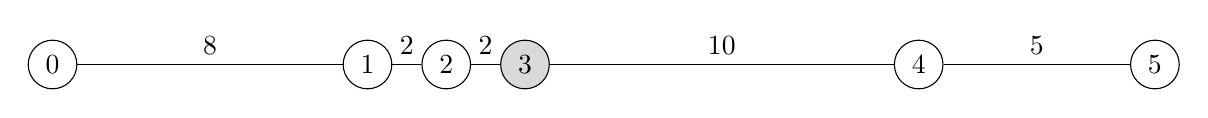
\begin{tikzpicture}
         % Define nodes
         \node[circle, draw, ] (0) at (0,0) {0};
         \node[circle, draw,] (1) at (4,0) {1};
         \node[circle, draw,] (2) at (5,0) {2};
         \node[circle, draw, fill=gray!30] (3) at (6,0) {3};
         \node[circle, draw,] (4) at (11,0) {4};
         \node[circle, draw,] (5) at (14,0) {5};
       
         % Draw edges
         \draw[-] (0) -- (1) node[midway, above] {8};
         \draw[-] (1) -- (2) node[midway, above] {2};
         \draw[-] (2) -- (3) node[midway, above] {2};
         \draw[-] (3) -- (4) node[midway, above] {10};
         \draw[-] (4) -- (5) node[midway, above] {5};
       \end{tikzpicture}
\end{soln}

\ifsolutions
\input{q4a-sol.tex}
\fi

\clearpage
\question[2]
Consider the following greedy algorithm.

\vspace{.1in}

\begin{algorithmic}[1]
\Procedure{Greedy-Provisions}{$d$, $p$, $R[1..k]$}
\State $i \leftarrow 0$ \Comment 0 is the starting town
\State $L \leftarrow$ empty list
\While {$i < k$}
\State
   \Comment find the town $j \le k$ that's furthest away from town $i$, among those of distance $\le dp$
   \State   $j \leftarrow i+1$
   \State   $d' \leftarrow R[j]$
      \While {($j < k$) and ($d' + R[j+1] \le dp$)}
         \State      $j \leftarrow j+1$
         \State      $d' \leftarrow d' + R[j]$
         \EndWhile
   \If {$j < k$}
      \State $L \leftarrow L$, $j$ \Comment append $j$ to the solution $L$
      \EndIf
   \State $i \leftarrow j$ \Comment update $i$
\EndWhile
\State output the list $L$
\EndProcedure
\end{algorithmic}
Explain why the output $L$ is a valid solution, i.e., one in which the hiker will
not run out of provisions, given that instance ($d,p,R[1..k])$ is 
guaranteed to have a valid solution.

\begin{soln}
   \begin{proof}
   We want to show that the list \( L \) given by \textsc{Greedy-Provisions} is a valid solution, which is 
   the distance between consecutive stops (or between the start and the first stop, or the last stop and the destination) 
   is at most \( dp \).
   
   At the beginning, the hiker is at town \( 0 \) with provisions 
   enough to travel \( dp \) kilometers. In each iteration of the while loop, 
   the algorithm sets the current town as \( i \) and then finds the furthest town \( j \) (with \( j\le k \)) 
   such that the total distance
   \[
   R[i+1] + R[i+2] + \cdots + R[j] \le dp.
   \]
   Since we are given that the instance \( (d,p,R[1..k]) \) has a valid solution, there is at least one 
   town reachable from town \( i \) within distance \( dp \). Therefore, the inner loop always terminates 
   with a valid choice of \( j \).
   
   If \( j < k \), the algorithm adds \( j \) to the list \( L \). This means that the distance from town \( i \) 
   to town \( j \) is at most \( dp \) kilometers long, ensuring that the hiker can safely travel to \( j \) 
   without running out of provisions. The algorithm then resets \( i \) to \( j \) and repeats.
   
   Finally, when the algorithm reaches a point where \( i = k \) (the hiker has reached the destination 
   or can reach it from the last chosen stop within \( dp \)), we have ensured that every distance of the journey 
   (from the start to the first stop, between consecutive stops, and from the last stop to the destination) 
   is at most \( dp \) kilometers.
   
   Thus, by always choosing the furthest reachable town in \( dp \) kilometers, 
   the algorithm make sure that the hiker never face situations where their travel distance is longer than what their provisions allow. 
   Therefore, the list \( L \) produced by \textsc{Greedy-Provisions} is indeed a valid solution.
   \end{proof}
\end{soln}
   

\ifsolutions
\input{q4b-sol.tex}
\fi

\question[3]
Give a big-$O$ bound on the running time of the greedy algorithm as a function of $k$, the number of towns, and justify your answer. (The lines of pseudocode above are numbered so that you can refer to specific lines in your reasoning.)

\begin{soln}
   \begin{proof}
   Let \( n = k \) denote the number of towns. We will see the running times below:
   
   \begin{itemize}
       \item The outer while loop (line 4) runs as long as \( i < k \). In each 
       iteration, the algorithm sets \( j = i+1 \) (line 6) and then uses the inner while 
       loop (lines 8--11) to extend \( j \) as far as possible such that the total distance 
       from town \( i \) to town \( j \) is at most \( dp \). 
       \item In the inner loop, each iteration increments \( j \) by 1 (line 9), and the 
       sum \( d' \) is updated in constant time (line 10). Since \( j \) can never exceed \( k \), 
       the total number of iterations of the inner loop across the entire execution is at most \( k \).
       \item The outer loop itself moves the current position \( i \) to \( j \) (line 13), so even 
       though the outer loop might iterate several times, each town is considered at most once in the inner loop. 
   \end{itemize}
   
   Since all operations within both loops (arithmetic operations, comparisons, and list appends at line 12) 
   are performed in constant time, the overall running time is \( O(k) \).
   
   Thus, the greedy algorithm runs in \( O(k) \) time.
\end{proof}
\end{soln}


\ifsolutions
\input{q4c-sol.tex}
\fi

\clearpage
\question[3]
Let $L$ be the output of the greedy algorithm, and let $i_1$ be the
first town in list $L$.  Let $L^*$ be an optimal solution for instance
$(d,p,R[1..k])$, and let $i_1^*$ be the first town in list $L^*$.  Let
$L'$ be the list obtained from $L^*$ by replacing $i_1^*$ by $i_1$.
Explain why $L'$ is also an optimal solution for instance
$(d,p,R[1..k])$.

\begin{soln}
   \begin{proof}
   Let \( L^* = \left( i_1^*, i_2^*, \dots, i_r^* \right) \) 
   be an optimal solution, so that each segment of the trip 
   (from the start to \( i_1^* \), from \( i_1^* \) to \( i_2^* \), etc.) has 
   total distance at most \( dp \). In particular, the distance from town 
   \( 0 \) to town \( i_1^* \) is at most \( dp \).
   
   The greedy algorithm selects \( i_1 \) as the farthest town reachable from 
   the start while still keeping the distance within \( dp \). Thus, 
   by definition we have that
   \[
   \text{distance}(0, i_1) \ge \text{distance}(0, i_1^*),
   \]
   with the guarantee that \(\text{distance}(0, i_1) \le dp\).
   
   Now, consider the list \( L' \) obtained from \( L^* \) by replacing \( i_1^* \)
    with \( i_1 \). Since \( i_1 \) is at least as far along the route as \( i_1^* \), 
    the following hold:
   \begin{enumerate}
       \item The segment from the start (town 0) to \( i_1 \) is at most \( dp \) (by the greedy selection).
       \item For the remaining part of the route, observe that any segment in \( L^* \) 
       following \( i_1^* \) was chosen so that the distance from \( i_1^* \) to the next 
       provision town (or destination) is at most \( dp \). Since \( i_1 \) is further along 
       than \( i_1^* \), the remaining segments, when shifted to start at \( i_1 \) instead 
       of \( i_1^* \), still have distances that do not exceed \( dp \). (This is because if 
       there were any issue with the segment from \( i_1 \) to the next stop, it would contradict 
       the validity of \( L^* \) or the fact that the greedy algorithm extended as far as possible 
       in the first move.)
   \end{enumerate}
   
   Thus, the modified list \( L' \) remains a valid solution. Moreover, since \( L' \) 
   has the same number of stops as \( L^* \), it is also an optimal solution.
   
   In summary, replacing \( i_1^* \) with \( i_1 \) does not increase the number of stops or the 
   length of any segment; hence \( L' \) is an optimal solution for the instance \((d,p,R[1..k])\).
   \end{proof}
\end{soln}
   

\ifsolutions
\input{q4d-sol.tex}
\fi

\question[3]
Complete the following argument that uses induction on $k$ to show that the greedy algorithm
outputs an optimal solution
 on any instance $(r,p,R[1..k])$ with a valid solution. You need to fill in the details for 
the base case, and parts (i) and (ii) of the inductive step. (The inductive hypothesis is done for you.)

\vspace{.1in}

\noindent
{\bf Base case}: If $k = 1$ then...

\ifsolutions
\input{q4e-sol.tex}
\fi

\noindent
{\bf Inductive hypothesis}: Let $k\ge 1$.
The greedy algorithm outputs an optimal solution for any instance with $k+1$ towns (assuming that the instance has a valid solution).

\noindent
{\bf Inductive step}: Show that the greedy algorithm outputs an optimal
solution when there are $k+2$ towns along the route. (Refer back to earlier parts of this problem.)

(i) There is an optimal solution that starts with $i_1$ because ...

\ifsolutions
\begin{soln}
...the solution $L'$ constructed in part 4 is such a solution.
\end{soln}
\fi

(ii) Once $i_1$ is added to the list, the remaining solution chosen by the Greedy algorithm is optimal because...

\ifsolutions
\input{q4f-sol.tex}
\fi

\vspace{.1in}

Combining (i) and (ii), we can conclude that our algorithm finds an optimal solution for instance
$(d,p,R[1..k])$.

\begin{soln}
   \noindent
   \textbf{Base case:}  
   If \( k = 1 \), there are two towns: town \( 0 \) (the start) and town \( 1 \) (the destination).
    The inter-town distance is \( R[1] \).  
   The greedy algorithm checks whether this distance is less than or equal to \( dp \). 
   Since the instance has a valid solution, we are guaranteed that \( R[1] \le dp \). 
   Then, no provision stop is needed, and the greedy algorithm outputs 
   the empty list as the solution. Thus, the base case holds.
   
   \vspace{0.2cm}
   \noindent
   \textbf{Inductive step:}  
   Assume that the greedy algorithm outputs an optimal solution for any 
   instance with \( k+1 \) towns (i.e., \( k \) inter-town distances), 
   given a valid solution. We must show that the greedy algorithm also
    outputs an optimal solution for an instance with \( k+2 \) towns.
   
   \vspace{0.2cm}
   (i) \textbf{There is an optimal solution that starts with \( i_1 \) because...}  
   Recall from part 4 that \( i_1 \) is the farthest town from town \( 0 \) 
   reachable within a distance of at most \( dp \). By the argument in part 4, 
   we can replace the first stop of any optimal solution with \( i_1 \) without 
   losing our optimal solution, 
   forming a new solution \( L' \). Therefore, 
   there exists an optimal solution that starts with \( i_1 \).
   
   \vspace{0.2cm}
   (ii) \textbf{Once \( i_1 \) is added to the list, the remaining solution chosen 
   by the Greedy algorithm is optimal because...}  
   By the greedy algorithm's design, after selecting \( i_1 \), the remaining 
   instance has only \( k+1 \) towns (from \( i_1 \) to the destination). By the 
   inductive hypothesis, the greedy algorithm finds an optimal solution for this
    reduced instance. Thus, the remaining solution is also optimal.
   
   \vspace{0.2cm}
   \noindent
   \textbf{Conclusion:}  
   Combining (i) and (ii), we can conclude by induction that the greedy algorithm finds an 
   optimal solution for any instance \((d, p, R[1..k])\) with a valid solution.
\end{soln}
   

\end{questions}




\end{document}
